\documentclass[article]{jss}
\usepackage[utf8]{inputenc}

\author{
Bastiaan Quast\\The Graduate Institute, Geneva \And Matthieu Stigler\\UC Davis
}
\title{\pkg{rddtools}: tools for Regression Discontinuity Design in R}
\Keywords{RDD, Regression, Discontinuity, Design, \proglang{R}}

\Abstract{
The rddtools package implements functions for handling Regression
Discontinuity Design in R.
}

\Plainauthor{Bastiaan Quast, Matthieu Stigler}
\Plaintitle{rddtools: tools for Regression Discontinuity Design in R}
\Shorttitle{\pkg{rddtools}}
\Plainkeywords{RDD, Regression, Discontinuity, Design R}

%% publication information
%% \Volume{50}
%% \Issue{9}
%% \Month{June}
%% \Year{2012}
%% \Submitdate{2012-06-04}
%% \Acceptdate{2012-06-04}

\Address{
    Bastiaan Quast\\
  The Graduate Institute, Geneva\\
  Maison de la paix Geneva, Switzerland\\
  E-mail: \href{mailto:bquast@gmail.com}{\nolinkurl{bquast@gmail.com}}\\
  URL: \url{http://qua.st/}
      Matthieu Stigler\\
  UC Davis\\
  California\\
  E-mail: \href{mailto:matthieustigler@gmail.com}{\nolinkurl{matthieustigler@gmail.com}}\\
  URL: \url{https://matthieustigler.github.io/}
  }

\usepackage{amsmath}

\begin{document}

\section{Introduction}\label{introduction}

The \texttt{rddtools} package\ldots{}

\section{Design}\label{design}

The package includes the following functions.

\section{Application}\label{application}

we use the data from the Initiative Nationale du Development Humaine
(INDH) a development project in Morocco. The data is included with the
\texttt{rddtools} package under the name \texttt{indh}.

We start by loading the package.

\begin{CodeChunk}
\begin{CodeInput}
library(rddtools)
\end{CodeInput}
\begin{CodeOutput}
Loading required package: AER
Loading required package: car
Loading required package: lmtest
Loading required package: zoo

Attaching package: 'zoo'

The following objects are masked from 'package:base':

    as.Date, as.Date.numeric

Loading required package: sandwich
Loading required package: survival
\end{CodeOutput}
\begin{CodeOutput}
Warning: package 'survival' was built under R version 3.2.1
\end{CodeOutput}
\begin{CodeOutput}
Loading required package: np
Nonparametric Kernel Methods for Mixed Datatypes (version 0.60-2)
[vignette("np_faq",package="np") provides answers to frequently asked questions]
IMPORTANT, this is an ALPHA VERSION
                        many changes to the API will follow
\end{CodeOutput}
\end{CodeChunk}

We can now load the included data set.

\begin{CodeChunk}
\begin{CodeInput}
data("indh")
\end{CodeInput}
\end{CodeChunk}

Now that we have loading the data we can briefly inspect the structure
of the data.

\textbackslash{}begin\{CodeChunk\}

\begin{CodeInput}
str(indh)
\end{CodeInput}

\textbackslash{}begin\{CodeOutput\} `data.frame': 729 obs. of 3
variables: \$ choice\_pg: int 0 1 1 1 1 1 0 1 0 0 \ldots{} \$ commune :
num 30.1 30.1 30.1 30.1 30.1 \ldots{} \$ poverty : num 30.1 30.1 30.1
30.1 30.1 \ldots{} - attr(\emph{, ``na.action'')=Class `omit' Named int
{[}1:11{]} 58 289 290 291 292 293 294 295 296 297 \ldots{} .. ..-
attr(}, ``names'')= chr {[}1:11{]} ``58'' ``289'' ``290'' ``291''
\ldots{} \textbackslash{}end\{CodeOutput\}
\textbackslash{}end\{CodeChunk\}

The \texttt{indh} object is a \texttt{data.frame} containing 729
observations (representing individuals) of three variables:

\begin{itemize}
\itemsep1pt\parskip0pt\parsep0pt
\item
  \texttt{choice\_pg}
\item
  \texttt{commune}
\item
  \texttt{poverty}
\end{itemize}

The variable of interest is \texttt{choice\_pg}, which represent the
decision to contibute to a public good or not. The observations are
individuals choosing to contribute or not, these individuals are
clustered by the variable \texttt{commune} which is the municiple
structure at which funding was distributed as part of the INDH project.
The forcing variable is \texttt{poverty} which represents the number of
households in a commune living below the poverty threshold. As part of
the INDH, commune with a proportion of household below the poverty
threshhold greater than 30\% were allowed to distribute the funding
using a \textbf{Community Driven Development} scheme. The cutoff point
for our analysis is therefore \texttt{30}.

We can now transform the \texttt{data.frame} to a special
\texttt{rdd\_data} \texttt{data.frame} using the \texttt{rdd\_data()}
function.

\begin{CodeChunk}
\begin{CodeInput}
rdd_dat_indh <- rdd_data(y=choice_pg,
                         x=poverty,
                         data=indh,
                         cutpoint=30 )
\end{CodeInput}
\end{CodeChunk}

The structure is similar but contains some additional information.

\begin{CodeChunk}
\begin{CodeInput}
str(rdd_dat_indh)
\end{CodeInput}
\begin{CodeOutput}
Classes 'rdd_data' and 'data.frame':    729 obs. of  2 variables:
 $ x: num  30.1 30.1 30.1 30.1 30.1 ...
 $ y: int  0 1 1 1 1 1 0 1 0 0 ...
 - attr(*, "hasCovar")= logi FALSE
 - attr(*, "labels")= list()
 - attr(*, "cutpoint")= num 30
 - attr(*, "type")= chr "Sharp"
\end{CodeOutput}
\end{CodeChunk}

In order to best understand our data, we start with an exploratory data
analysis using tables\ldots{}

\begin{CodeChunk}
\begin{CodeInput}
summary(rdd_dat_indh)
\end{CodeInput}
\begin{CodeOutput}
### rdd_data object ###

Cutpoint: 30 
Sample size: 
    -Full : 729 
    -Left : 371 
    -Right: 358
Covariates: no 
\end{CodeOutput}
\end{CodeChunk}

\ldots{}and plots.

\begin{CodeChunk}
\begin{CodeInput}
plot(rdd_dat_indh[1:715,])
\end{CodeInput}


\begin{center}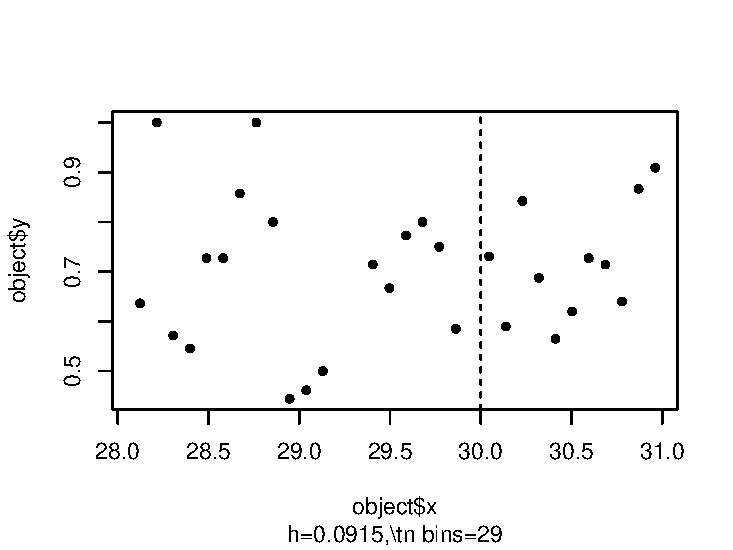
\includegraphics{README_files/figure-latex/unnamed-chunk-7-1} \end{center}

\end{CodeChunk}

We can now continue with a standard Regression Discontinuity Design
(RDD) estimation.

\begin{CodeChunk}
\begin{CodeInput}
(reg_para <- rdd_reg_lm(rdd_dat_indh, order=4))
\end{CodeInput}
\begin{CodeOutput}
### RDD regression: parametric ###
    Polynomial order:  4 
    Slopes:  separate 
    Number of obs: 729 (left: 371, right: 358)

    Coefficient:
  Estimate Std. Error t value Pr(>|t|)
D  0.26428    0.16590   1.593   0.1116
\end{CodeOutput}
\end{CodeChunk}

and visualising this estimation.

\begin{CodeChunk}
\begin{CodeInput}
plot(reg_para)
\end{CodeInput}


\begin{center}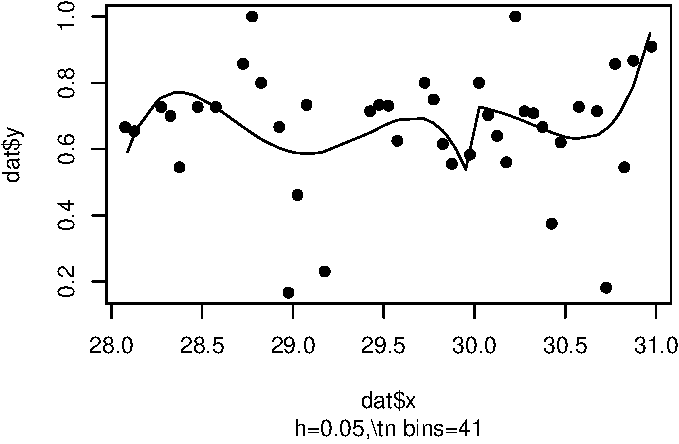
\includegraphics{README_files/figure-latex/unnamed-chunk-9-1} \end{center}

\end{CodeChunk}

In addition to the parametric estimation, we can also perform a
non-parametric estimation.

\begin{CodeChunk}
\begin{CodeInput}
bw_ik <- rdd_bw_ik(rdd_dat_indh)
(reg_nonpara <- rdd_reg_np(rdd_object=rdd_dat_indh, bw=bw_ik))
\end{CodeInput}
\begin{CodeOutput}
### RDD regression: nonparametric local linear###
    Bandwidth:  0.7812904 
    Number of obs: 467 (left: 146, right: 321)

    Coefficient:
  Estimate Std. Error z value Pr(>|z|)  
D 0.178174   0.095319  1.8692  0.06159 .
---
Signif. codes:  0 '***' 0.001 '**' 0.01 '*' 0.05 '.' 0.1 ' ' 1
\end{CodeOutput}
\end{CodeChunk}

and visualising the non-parametric estimation.

\begin{CodeChunk}
\begin{CodeInput}
plot(reg_nonpara)
\end{CodeInput}


\begin{center}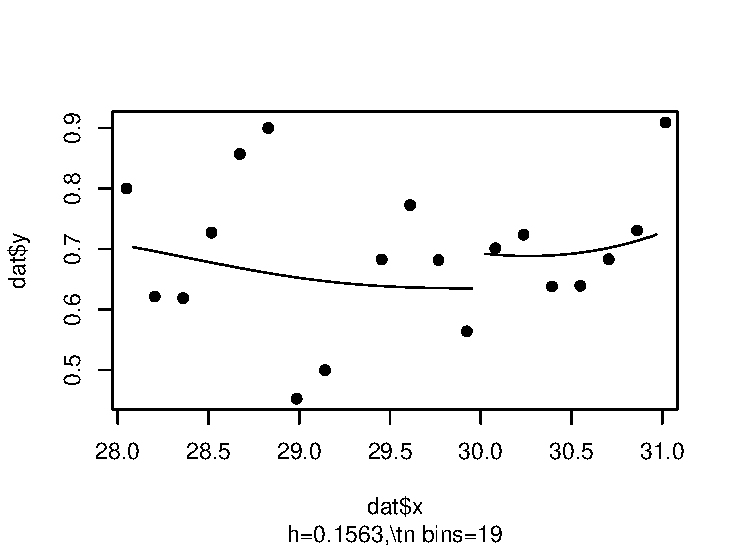
\includegraphics{README_files/figure-latex/unnamed-chunk-11-1} \end{center}

\end{CodeChunk}

Sensitity tests.

\begin{CodeChunk}
\begin{CodeInput}
plotSensi(reg_nonpara, from=0.05, to=1, by=0.1)
\end{CodeInput}


\begin{center}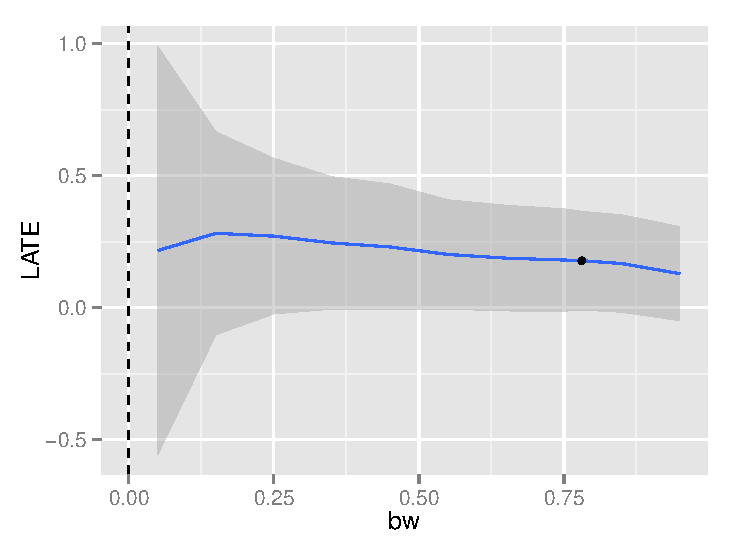
\includegraphics{README_files/figure-latex/unnamed-chunk-12-1} \end{center}

\end{CodeChunk}

\section{References}\label{references}

\end{document}

